\documentclass[letterpaper,twocolumn,10pt]{article}
\usepackage{usenix,epsfig,endnotes}
\usepackage[utf8]{inputenc}
\usepackage{color}
\usepackage{graphicx}


\newcommand{\kyle}[1]{\textcolor{blue}{[[\textsf{Kyle:  #1}]]}}
\newcommand{\fan}[1]{\textcolor{red}{[\textsf{Fan:  #1}]}}
\newcommand{\ari}[1]{\textcolor{green}{[\textsf{Ari:  #1}]}}

%don't want date printed
\date{}

%make title bold and 14 pt font (Latex default is non-bold, 16 pt)
\title{\Large \bf Town Crier}

%for single author (just remove % characters)
\author{
{\rm Your N.\ Here}\\
Your Institution
\and
{\rm Second Name}\\
Second Institution
\and
{\rm Name}\\
Name Institution
} % end author


\begin{document}
\maketitle

% Use the following at camera-ready time to suppress page numbers.
% Comment it out when you first submit the paper for review.
% \thispagestyle{empty}

\subsection*{Abstract}
Your Abstract Text Goes Here.  Just a few facts.
Whet our appetites.

\section{Introduction}

\section{Identifying Client Contracts}
The Authenticated Data Feed (ADF) needs some method to identify and serve prospective clients.  There are two on-chain methods: registration and client flags.  The registration method requires an additional transaction and will therefore incur an additional fee.  The flags method must scan all contracts at every block update to support dynamic data requests.  It may therefore be useful to support both methods, using the blockchain crawler for one-time requests and registration for more complicated contracts, depending on the resource costs of the crawler.
\subsection{Registration / Explicit Requests for Data}
	This requires the client to initiate communication to the ADF with a \emph{Initial Client Request} message, which consists of a (potentially zero-value) transaction to the ADF address with a message specifying what signed data it wants. 
	
\subsection{Client Flags / ADF Blockchain Crawler}
	This method requires only that the client contract has in its key/value store a flag indicating its request for service from the ADF and the specifics of the data it wants.  The ADF can then crawl the blockchain looking for contracts with this specific flag set and read the data requested.
	
\subsection{Off Chain Communication}
	The ADF may be notified of prospective clients by any manner of off-chain communication however there will be no public record of this request.  The ADF may then selectively deny service.  Malicious clients may also have an easier time flooding the ADF with requests, compared to the other two methods which have an Ether cost (contract creation).\\

\subsection{Migration Path}

Ultimately, we expect sources themselves to act as ADFs. The migration path is : (1) Town Crier; (2) XML labels on data; (3) Integration of Town Crier features into source directly

\section{Trusted Hardware}
Placeholder: Intel SGX~\cite{anati2013innovative,sgxmanual} is a
soon-to-be-released trusted hardware.

\section{Architecture}

\begin{figure*}[h]
\centering
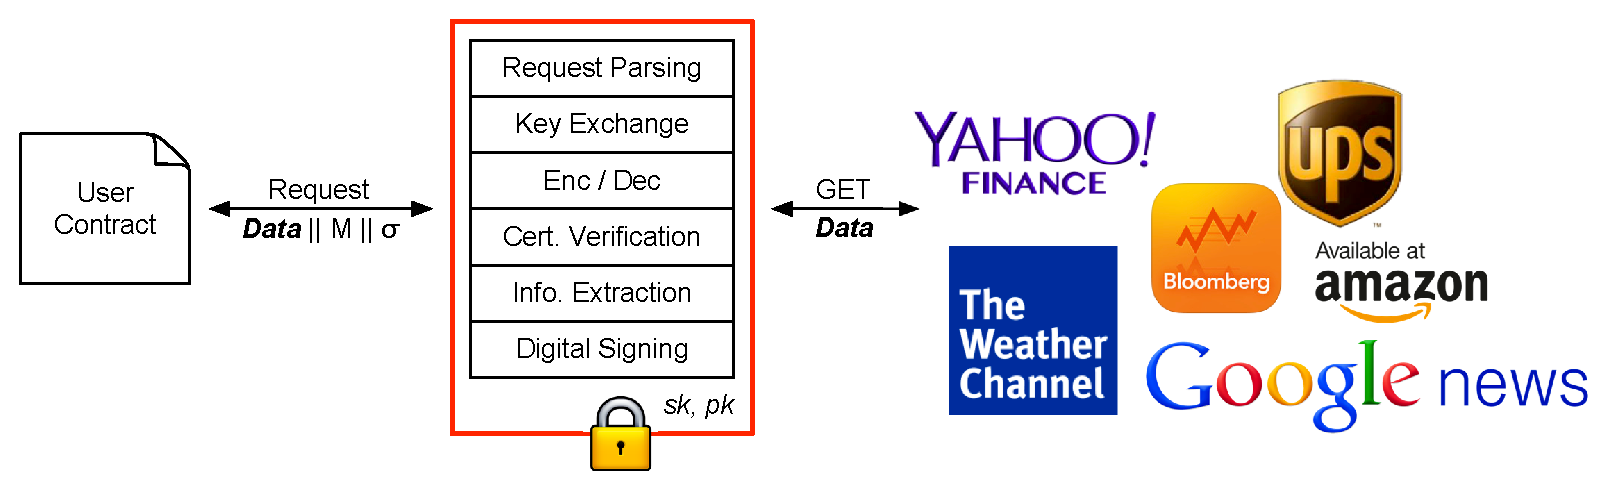
\includegraphics[width=\textwidth]{figures/arch}
\caption{Town Crier Architecture}
\label{fig:arch}
\end{figure*}


\section{Payment Methods}	
\subsection{Separate Fair Exchange Contracts}
    The ADF or the client contract creates or uses an existing \emph{fair exchange contract} for each data request.  This contract requires input from the client in the form of some amount of Ether (this can happen during the creation of the contract), and the signed data from the ADF.  Once both inputs have been received, the contract sends the Ether to the ADF and the data to the client. Note the client should send the currency first as once the ADF publishes the signed data it will be publicly visible (unless we use zero-knowledge proofs). If the ADF fails to deliver the data within a time period then the client's money is refunded.\\
    \indent The main benefit of this method is that the fair exchange contract should be easier to verify for both parties.  Depending on the specifics of the attestation it needs to check, it may be possible for the contracts to be completely templated.  Also note that creating a new contract will incur a transaction fee.  These data fair exchange contracts can potentially batch data requests and verification and can be re-used for subsequent requests if desired. 
    
    \kyle{This is my thought as well.  A client may extract the address, pricing info, and a code template for fair exchange from the ADF website.  The issue I was trying to get at was that verifying the bytecode of one function in a contract may be more difficult than simply verifying an entire contract's bytecode due to having to isolate the function.  I don't know whether isolating a function is hard or if the bytecode may change depending on the client contract (offsets, compilers, etc), but at the very least it involves the extra step of checking the function entry point in addition to simply matching the hash of the bytecode}
    
\subsection{Payment Built-in to the Client Contract}
    The client contract includes a function that accepts signed data and pays out the specified amount of coins to the sender if the data is correct.  This requires the ADF to verify the correctness of the function and that the client has sufficient funds.  It would be potentially useful for this function to be templated for ease of use and verification, and at the very least it needs to conform to some specification agreed upon by the client and ADF. 
    
\subsection{Payment built-in to the ADF}
    The client may send payment directly to an ADF contract as part of its initial request.  The ADF contract code must maintain a list of clients and their corresponding requests.  It must also verify the attestation on the data before forwarding it to the client since it has already been paid.  The client must verify that the ADF contract code is correct.
    
\fan{Do all of 9 combinations of (2.1, 2.2, 2.3) and (3.1, 3.2, 3.3) make sense? Or we should point out the best combinations?}
\kyle{All combinations make sense to me with the exception of client flags and payment built-in to the ADF (2.2, 3.3)}
    
\section{Privacy}
Everything posted to the blockchain is publicly visible, including all data requests directed towards the ADF.  It is possible to encrypt data requests, as the ADF may decrypt and process them off-chain.  It is not always possible to encrypt the responses, as the contract requesting the data will often need to process the data.

\subsection{Privacy From Peers}
    In some cases clients may want to keep their requests for data private.  For example a client requesting information about the weather may need to provide his zip code for accurate local results.  However he may not wish for his zip code to be publicly visible.  To solve this, he may encrypt his zip code (or his entire request) with the ADF's public key before posting it to the blockchain.  Note that all encryption and decryption operations can be done off-chain to avoid incurring excessive gas fees.\\

\subsection{Partial Privacy From ADFs}
    Clients may also wish to keep some information private from the ADF.  Consider again a client requesting information about the weather who wishes to keep his zip code private not only from the public, but from the ADF as well.  This can be accomplished by utilizing two ADFs $A_1$ and $A_2$.  The client creates $n-1$ randomized decoy requests for data along with his actual request.  He orders these requests such that his actual request appears at a randomly chosen index $i$.  He then encrypts all requests under the public key of $A_1$ and submits all $n$ encryptions in order to $A_1$.  He encrypts $i$ under the public key of $A_2$ and submits the encryption to $A_2$.  $A_1$ decrypts and computes the results for all $n$ queries and submits the results to $A_2$.  $A_2$ returns to the client the $i$th result.  So long as the two ADFs do not collude (in the context of the weather example, this means neither ADF can know both the zip codes and the index $i$), $A_1$ can only guess the clients true data with probability $\frac{1}{n}$.  \kyle{There is definitely some leakage here if the response returned by $A_2$ is in plaintext} 
    
    
    \kyle{The issue is that the information has to appear in plaintext somewhere on the blockchain in order for a contract to use it, otherwise $A_2$ could simply encrypt the response under the public key of the client.  We could obfuscate the result with a mask, but the client contract will still need to unmask the data to use it, and when it does anyone can read it.  Then in our example $A_1$ knows what the weather was at the clients zipcode and may cross reference with the zipcodes he was given}
    \ari{As regards leakage, that's right. If the output of the contract depends on the zip code, information will leak}
    \ari{Remember the compression trick as well. Let $G$ be an additive group over 5-decimal-digit numbers. Let $PRF_k: \{0,1\}^{*} \rightarrow G$ be a PRF. To send a correct zip code $z$ in list of $n$ zip codes, of which $n-1$ are ``decoys'', the client selects a key $k$ and index $i \in [1,n]$ at random. The client sends $(k,p = PRF_k[i] - z)$. The ADF decodes the list as $\{PRF_k[1] - p, \ldots, PRF_k[n]  - p\}$.}

\subsection{Fully Private Requests}
    If a client wishes to keep the entirety of the request private, he may do so by leveraging the ADF's trusted hardware.  The initial request is encrypted under a public key stored in the trusted hardware, which processes the request.  A malicious ADF operator may only determine the sources which are contacted as a result of the request, and if necessary these can be masked with decoy queries as well.

\subsection{Decoy Requests}
Decoy requests for partially private protocols should be in the same class as the real request.  In the weather example, all zipcodes provided as decoy requests should be experiencing the same weather as in the actual request.  As the outcome of the contract is public, the ADF will be able to determine the value of the weather at the client's zipcode and can discount all decoys that do not match.\\\\
If the class of decoy requests can be pseudorandomly generated, we can save data transmission fees by sending only a random function, a seed, and a mask to ensure that the real request is computed.

\section{Example: Travel Insurance}
An insurance company may provide insurance for canceled flights by maintaining an Ethereum contract on the blockchain.  The source code of this contract should be public to allow potential customers to verify its correctness.  A customer may then purchase insurance by paying a predetermined amount of ether into the contract.  In addition, this transaction should include identifying information (flight number) for the flight for which the customer wishes to be insured.  However, the customer may wish to hide the flight number in order to avoid publicly revealing which flight he/she will be on.  To achieve this, the customer may encrypt the flight number under a public key whose corresponding private key is stored only in the ADF's trusted hardware.  Thus only enclave code will be able to view the unencrypted flight number, preventing even a malicious ADF or data center operator from compromising privacy. Once the ADF is made aware of the requests (as detailed in section 2), it proceeds by decrypting the flight number and determining whether or not the relevant flight was canceled. It strips all identifying information from response, and returns either ``Canceled'' or ``Not canceled.''  

\section{Applications}


\begin{itemize}
\item micro-insurance:
    \begin{itemize}
    \item weather
    \item item delivery
    \item flight delay (note: something we could implement easily ourselves...)
    \end{itemize}
\item Ethereum and USD exchange
\item stock price
\item BTC exchange (with and without ADF)
\item Simple derivatives
\item sports betting
\end{itemize}

\section{Kyle's tasks for week of 7 Dec.}
\begin{enumerate}
\item specifications for end-to-end private requests (microtransactions, travel insurance)\\
-hiding in a crowd, same class of decoy queries\\
-encrypt queries and offchain computation \\
-consider information leaked from which party gets paid
\item webcrawler
\item Explain choice of subscription model, design considerations; discuss possible entry-point templates
\item Think about IoT applications of ADFs
\end{enumerate}

\section{Fan's tasks for week of 7 Dec.}
\begin{itemize}
\item Look into trusted time source 1) based on PCH clock or 2) TLS timeout+connection to trustworthy time source
\item TCB for ADF
\item Test OpenSGX
\begin{itemize}
\item Check cert for TLS connection
\item Extract data from target
\item Handle encrypted queries and encrypted replies
\item Think about IoT applications of ADFs
\end{itemize}
\end{itemize}

{\footnotesize \bibliographystyle{acm}
\bibliography{sgx.bib}}

\end{document}
